\chapter{Классификация существующих решений}

В данном разделе описываются существующие метрики качества упрощенного текста, предлагаются критерии оценки методов упрощения. Затем описываются известные решения поставленной задачи и приводится их классификация по сформулированным критериям.

\section{Метрики}

Оценка качества упрощения текста - довольно субъективная задача, трудно переводимая на язык компьютера. Поэтому до сих пор предпочтение отдается человеку, который оценивает упрощенное предложение с точки зрения его грамматической корректности, сохранения смысла и простоты, используя шкалы Лайкерта\footnotemark{}. Однако тенденция к использованию технологии обучения без учителя потребовала адаптации уже существующих показателей для автоматической оценки качества упрощения или разработки новых метрик.\footnotetext{Шкала Лайкерта - это ординальная (порядковая) шкала ответов на вопрос или утверждений, расположенных в иерархической последовательности, например, от «полностью согласен» через «затрудняюсь ответить» и до «категорически не согласен»\cite{likert}.}


\subsection{Индексы удобочитаемости}
Индексы удобочитаемости используются в США для присвоения любому тексту уровня его <<простоты>>. Обычно для такой оценки применяется сразу несколько формул, которые учитывают количество предложений, слогов, общее количество слов и количество редких слов в рассматриваемом тексте. Отличаются эти формулы лишь коэффициентами, расположением членов в формуле или способом интерпретации результата.

Например, в тесте Флэша-Кинкайда предполагается, что чем меньше слов в предложениях и чем короче слова, тем более простым является текст. В результате применения формулы \ref{eq:1} корпус получает оценку, по которой с помощью специальной таблицы интерпретируется уровень образования, необходимый для понимания текста\cite{test}.

\begin{eqnarray} 
	\label{eq:1}
	206.835 - 1.015 \cdot \left(\frac{\textrm{количество слов}}{\textrm{количество предложений}}\right) - \notag\\ - 84.6 \cdot \left(\frac{\textrm{количество слогов}}{\textrm{количество слов}}\right) 
\end{eqnarray}


Основной недостаток индексов удобочитаемости заключается в том, что используемые в них формулы <<поощряют>> короткие предложения с простыми словами, но не способны распознавать грамматически неправильные результаты или упрощенные предложения, некорректно передающие смысл исходного.

\subsection{SARI}

Метрика SARI (\textbf{s}ystem output \textbf{a}gainst \textbf{r}eferences and against the \textbf{i}nput sentence - результат системы против эталонного решения и исходного предложения) была разработана в 2016 году специально для задачи упрошения и в настоящее время считается наиболее применимой\cite{xu_optimizing_2016}.

Авторы SARI заметили, что, в отличие от метрик качества машинного перевода, где исходное предложение записано на другом языке, метрики качества упрощения могут использовать еще один источник для оценки результирующего предложения - само исходное предложение, так как оно записано на том же языке, что и упрощенное. Разработанная ими метрика напрямую оценивает, насколько корректно были выбраны слова, которые были добавлены, удалены или же сохранены моделью.

Результаты исследования авторов показали высокую корреляцию оценки метрикой SARI с оценками качества упрощения человеком, однако, эта функция требует нескольких <<справочных>> примеров упрощения, которые не всегда доступны. Более того, она более сфокусирована на оценке упрощения на уровне лексики, и слабо способна распознать степень того, насколько проще стало предложение на уровне его структуры.

\subsection{SAMSA}

Метрика SAMSA (\textbf{s}implification \textbf{a}utomatic evaluation \textbf{m}easure through \textbf{s}emantic \textbf{a}nnotation, (автоматическая оценка упрощения с помощью семантической аннотации), разработанная в 2018 году, была призвана исправить последний недостаток SARI, то есть оценивать как качество лексического упрощения, так и простоту полученного предложенияя с точки зрения его структуры\cite{sulem_semantic_2018}.

SAMSA предполагает, что оптимальное разделение исходного предложения - это такое, при котором каждой структуре подлежащее-сказуемое присваивается собственное предложение, и измеряет, в какой степени это утверждение справедливо для рассматриваемой пары ввода-вывода, используя семантическую структуру. Эта метрика фокусируется на основных семантических компонентах предложения и менее внимательно относится к удалению других структурных единиц.

Авторы SAMSA также демонстрируют высокую корреляцию оценки этой метрикой с оценками качества упрощения человеком. Но так как SAMSA появилась относительно недавно, она в настоящее время еще широко не используется. Более того, она не решила другую проблему SARI - потребность в <<справочных>> примерах упрощения.


\section{Критерии оценки решений}

Как уже упоминалось, данная работа фокусируется на поиске решения задачи упрощения в узком смысле, как на задаче получения более легкого для чтения и понимания текста за счет уменьшения его лексической и структурной сложности\cite{martin_muss_2021}. Поэтому в первую очередь рассматриваемые решения будут классифицироваться на те, что решают задачу упрощения в широком смылсе и те, что решают ее в узком смысле.

Из данного выше определения следует вывод, что упрощение можно условно разделить на лексическую и структурную составляющую. Поэтому другими критериями оценки могут стать ответы на вопросы, учитывает ли рассматриваемое решение каждую из составляющих.

Целью такой классификации будет поиск решения, которое работает с задачей упрощения текстов в узком смысле и при этом учитывает как лексическое, так и структурное упрощение предложений текста.

Ранее было приведено несколько метрик, которые способны автоматически оценивать качество упрощения. Однако решения, которые будут рассмотрены далее, обучались и тестировались на разных корпусах, оценивались разными метриками, то есть нет готовых данных для объективного сравнения решений по определенной метрике. В связи с ограниченным временем на выполнение работы, нет возможности самостоятельно получить эти данные. Поэтому классификация решений по их эффективности проводиться не будет.


\section{Подходы к решению задачи}

Глобально выделяют два подхода к решению задачи упрощения текстов - экстрактивный (извлекающий) и абстрактный.

Большинство ранних работ, посвященных задаче упрощения текстов, использовали экстрактивный подход - выделение в документе тех предложений, которые передают больше информации. Полученные тексты будут легче для чтения и восприятия, так как они становятся значительно короче исходных, а многие редко употребляемые слова будут отброшены, так как не попадут в выбранные предложения. 

Этот подход достаточно прост в реализации, однако он подходит лишь для решения задачи упрощения текстов в широком смысле, так как из-за удаления предложений, несущих малое количество информации, исходный смысл корпуса будет передан не в полной мере. Поэтому решения экстрактивного подхода в дальнейшем в данной работе рассматриваться не будут.

С ростом доступности вычислительных ресурсов и количества исследований в области NLP для решения задачи упрощения текстов все чаще стал использоваться абстрактный подход, подразумевающий \textbf{переписывание} передаваемого текста предложение за предложением\cite{see_get_2017}. 

\section{Решения абстрактного подхода}

Решения задачи упрощения текстов, относяшиеся к абстрактному подходу, можно разделить на два класса: те, что основаны на текстовых заменах, и те, что подразумевают генерацию нового текста.

\subsection{Текстовые замены}

Текстовые замены на уровне слов или целых фраз лежали в основах первых работ, посвященных абстрактному подходу к упрощению текстов \cite{paetzold_survey_2017}. Этот процесс фокусируется на сокращении лексического содержания текста, но не принимает во внимание такие подзадачи упрощения структурной составляющей, как грамматическое или синтаксическое упрощение\cite{shardlow_survey_2014}. Таким образом, эти решения не учитывают все аспекты решаемой задачи, и поэтому в дальнейшем в работе рассматриваться не будут.

\subsection{Генерация нового текста}
Современные решения абстрактного подхода,  включают в себя разбиение сложных предложений на более простые, удаление редко употребляемых слов и генерацию на этой основе нового текста. Это стало возможным благодаря появлению нейронных сетей, в частности, рекуррентных нейронных сетей (RNNs)\footnote{Рекуррентная нейронная сеть, или RNN, - это сеть, которая работает с последовательностью и использут собственные промежуточные выходные данные в качестве входных данных для последующих шагов \cite{noauthor_nlp_nodate}}, которые позволяют решать задачи <<от последовательности к последовательности>> (seq2seq)\footnote{Сеть sequence-to-sequence (<<от последовательности к последовательсности>>), или сеть seq2seq, или сеть кодировщика-декодера, представляет собой модель, состоящую из двух RNN, называемых кодировщиком и декодером. Кодер считывает входную последовательность и выдает один вектор, а декодер считывает этот вектор для создания выходной последовательности \cite{noauthor_nlp_nodate}}.

Последовательность действий в решении задач, сведенных к seq2seq, является универсальной. Предварительная обработка данных включает очистку входного и результирующего текста, удаление знаков препинания и специальных символов, формирование словаря типичных слов. Далее входные и результирующие предложения преобразуются в числовую форму с вектором одинаковой длины либо путем их усечения, либо путем их дополнения. Затем модель обучается, после чего новые поступающие данные также сначала векторизуются, преобразуются к определенной длине и упрощаются, а только после этого преобразовываются обратно из числовой формы в текстовую.

Далее будут рассмотрены различные виды решений задачи упрощения текста, относящиеся к классу тех, которые используют генерацию нового текста.

\subsubsection{Синтаксическое упрощение}

Цель синтаксического упрощения заключается в выявлении грамматически сложных частей текста и их переписывание для облегчения понимания. Такое упрощение может включать разделение длинных предложений на более короткие фрагменты, переписывание предложений со страдательным залогом так, чтобы в них использовался залог действительный\footnotemark{}, разрешение двусмысленностей и анафор\cite{shardlow_survey_2014}. По ходу выполнения синтаксического упрощения удается заменять слова, которые считаеются <<сложными>> из-за наложения морфем, участвующих в переводе слова из одной части речи в другую, на их более простые, оригинальные версии.

\footnotetext{
Действительный залог имеют глаголы переходные, обозначающие действие, производимое субъектом и активно направленное на объект. Действительный залог имеет синтаксическую характеристику: субъект действия является подлежащим, а объект - дополнением в винительном падеже без предлога: Мир победит войну.

Страдательный залог выражается присоединением к глаголам действительного залога аффикса -ся (ср.: Рабочие строят дома. - Дома строятся рабочими). Кроме того, значение страдательного залога может быть выражено формами страдательных причастий - полных и кратких. Например: Мать любима (любимая). Тема изучена (изученная)\cite{rus_pas}.
}

Основополагающей работой в области синтаксического упрощения была система автоматического создания правил переписывания предложений\cite{chandrasekar_automatic_1997}, которая брала аннотированные корпуса и изучала возможные принципы упрощения для конкретной предметной области.  

Более поздние работы по синтаксическому упрощению были сосредоточены на улучшении структуры выходного текста - обеспечении того, чтобы предложения появлялись в правильном порядке \cite{siddharthan_syntactic_2006}. Также этот подход стали использовать для распознавания именованных сущностей (Named Entity Recognition, NER), особенно в области медицины \cite{jonnalagadda_biosimplify_2010}.

Синтаксическое упрощение обычно выполняется в три этапа. Пример применения каждого этапа к предложению показан на рисунке \ref{fig:3steps}

\clearpage
\begin{figure}[h!]
	\begin{center}
		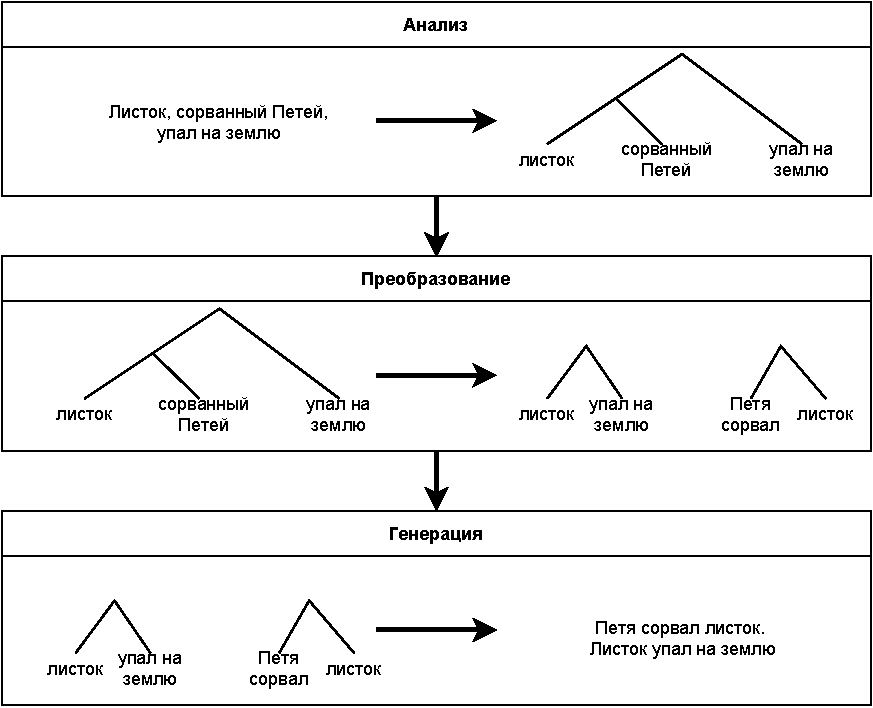
\includegraphics[pages=-, scale=0.9]{./inc/img/3steps_my.pdf}
		\caption{Три этапа синтаксического упрощения}  
		\label{fig:3steps}
	\end{center}
\end{figure}



\begin{enumerate}
	\item Анализ. Определяется структура предложения и созданется дерево синтаксического анализа. Это может быть сделано на разных уровнях детализации, но наилучшие результаты достигаются на довольно высоком уровне, когда слова и фразы группируются в так называемые <<супер-теги>>, представляющие собой фрагменты исходного предложения. Такие теги могут быть объединены по обычным грамматическим правилам и являются структурированной версией текста. На этом же этапе простой проверкой по заранее заданным правилам или с помощью бинарного классификатора SVM (метод опорных векторов)\cite{shardlow_survey_2014} определяется сложность предложения.
	%\footnotetext{<<Машина опорных векторов>> (Support Vector Machine, SVM) - это алгоритм машинного обучения с учителем, который в основном используется в задачах классификации. Каждая запись представляется в виде точки в n-мерном пространстве (где n - количество признаков), при этом значение каждого признака равно значению определенной координаты. Затем выполняется классификацию, в результате которой находится гиперплоскость, разделяющая два класса \cite{noauthor_svm_2017}.}
	
	\item Преобразование. Дерево синтаксического анализа модифицируется в соответствии с набором правил, которые выполняют операции упрощения. Например, разбиение сложного предложения на несколько более простых, перестановка или удаление полученных предложений\cite{hutchison_ernesta_2013}.
	
	\item Генерация. В текст вносятся дополнительные изменения для улучшения согласованности и удобства чтения, добавляются знаки препинания.
\end{enumerate}

Синтаксическое упрощение считалось важным компонентом систем упрощения текстов и было реализовано в системах, которые повсеместно используются как вспомогательные, например, в PSET\cite{alva} и Porsimples\cite{aluisio_fostering_2010}.

Преимущества синтаксического упрощения заключаются в его высокой точности и применимости к другим задачам NLP \cite{shardlow_survey_2014}. 

Недостатком является трудоемкость создания и проверки применимости правил перезаписи. Но в последнее время достижения в области методов глубокого обучения привели к автоматизации процесса обнаружения возможности применения синтаксического упрощения.

Еще один недостаток -  лексическое упрощение выполняется не в полной мере. По ходу выполнения синтаксического упрощения удается заменять лишь некоторые слова, которые были упомянуты выше, но не редкоупотребляемые и специализированные слова.


\subsubsection{Статистический машинный перевод}
Автоматизированный машинный перевод является устоявшейся техникой в NLP. Эта задача подразумевает автоматическое преобразование лексики и синтаксиса одного языка в правила другого, в результате чего получается переведенный текст. Машинный перевод был успешно применен\cite{shardlow_survey_2014} к задаче упрощения текстов путем ее переформулирования в задачу <<одноязычного перевода>>. То есть задача упрощения была сведена к переводу с исходного <<сложного>> языка на целевой <<простой>> язык.

Разновидностью машинного перевода является статистический машинный перевод (Statistical Machine Translation (SMT)), основанный на статистических моделях, которые изначально <<ничего не знают>> о правилах и лингвистике, а затем изучают большие объемы пар предложений из выровненных двуязычных корпусов, настраивая свои параметры (наиболее вероятный вариант перевода того или иного слова), а затем применяются к новым текстам. 

Например, модель для перевода с русского на английский изучила перевод одного предложения: <<Я вижу дом>> в <<I see a house>>. Если теперь запросить у нее перевод слова <<дом>>, она предположит, что слово с равной вероятностью переводится как <<I>>, <<see>>, <<a>> или <<house>>. Но если предоставить модели еще одно соответствие, что предложение <<Этот дом большой>> переводится как <<That house is big>>, то из анализа уже двух сопоставлений переводчик отметит, что в переводах все слова встретились по одному разу, а <<house>> — дважды, равно как и слово <<дом>> (и никакое другое) в исходных предложениях. А значит, по сравнению со всеми остальными вариантами увеличивается вероятность соответствия <<дом = house>> и между ними установилась связь. 

Задача перевода облегчается, когда исходный и целевой языки схожи, и для преобразования предложения требуется минимальное число изменений его структуры. И именно этот тип машинного перевода был применен к задаче упрощения текстов\cite{shardlow_survey_2014}.

%Практически системы часто используют и модифицируют стандартный инструмент SMT, такой как Moses [43], который был применен к задаче TS для английского языка [20]. Мозес был дополнен модулем удаления фраз, который удалял ненужные части сложного исходного текста с многообещающими результатами [76].


Эффективность применения статистического машинного перевода для задачи упрощения предложений в значительной степени зависит от набора данных, используемых для обучения модели. Например, если в них содержатся слишком длинные исходные предложения или упрощененные предложения слишком сильно оличаются по своей структуре от входных, то этот подход не позволит отслеживать и верно сопоставлять различные части предложений. Кроме того, данный метод не учитывает знаки препинания и разбиение сложных предложений, что зачастую приводит к потере контекста и получению структурно сложных предложений.


\subsubsection{Использование методов глубокого обучения}

Глубокое обучение - это разновидность машинного обучения, в которой нейронные сети и алгоритмы, основанные на структуре и функционировании человеческого мозга, обучаются на большом объеме данных для создания шаблонов принятия решений. Этот подход позволяет обучаться путем многократного выполнения задач и настройки модели для улучшения результата\cite{deep}.

Методы глубокого обучения после своего появления стали активно применяться для решения задачи упрощения текстов, сформулированной в терминах моделирования seq2seq. Однако в ранних моделях seq2seq были две существенные проблемы.

Во-первых, это неточность результата. Эффективность моделей кодировщика-декодера сильно зависит от расположения слов в исходном предложени, поэтому модель зачастую не может расположить редко употребляемые слова в корректную позицию выходного предложения. Один из вариантов решения этой проблемы -   добавление так называемых <<указателей>> на подобные слова в исходном тексте\cite{nisioi_exploring_2017}. Это решение показало многообещающие результаты в сохранении корректного смысла сгенерированного упрощенного текста.

Во-вторых, это повторения в выводе. Данная проблема часто возникает в простых моделях seq2seq из-за того, что так называемые <<стоп-слова>> (<<как>>, <<и>>, <<а>>, <<то>> и т. д.) встречаются в тексте намного чаще остальных, и модель учится чаще предсказывать их. В частности, именно эта проблема стала основным недостатком в решении, описанном ранее\cite{nisioi_exploring_2017}. Для борьбы с этим недостатком было предложено штрафовать модель за повторения с помощью введение векторов <<покрытия>>, <<внимания>> и <<контекста>>. Эти вектора отслеживают слова, которые перешли из исходного предложения в упрощенное: вектор <<внимания>> - слова, несущие основной смысл, <<контекста>> - сопуствующую информацию, <<покрытия>> - общий переданный объем слов. Именно вектор покрытия призван дополнительно контроллировать вектора  <<внимания>> и <<контекста>> и штрафовать модель при их наложении друг на друга\cite{see_get_2017}.

Также к задаче упрощенияя текстов было успешно применено глубокое обучение, дополненное обучением с подкреплением\cite{zhang_sentence_2017}. Была разработана модель кодировщика-декодера в сочетании с системой глубокого обучения с подкреплением DRESS (Deep Reinforcement Sentence Simplification, глубокое упрощение предложений с подкреплением), стремящаяся оптимизировать функцию потерь, которая поощряет простые, легко читаемые и сохраняющие исходный смысл результаты упрощения. Обучение с подкреплением позволяет генерировать сразу несколько вариантов результата, а затем выбирать из них наиболее удачный. С помощью этой модели было показано, что такое сочетание дает возможность для предоставления дополнительной (предварительной) информации в данные.

Основная проблема решений, использующих глубокое обучение, состоит в их большой ресурсоемкости, что ограничивает количество параметров в используемых в них моделях. Но появление языковой модели BERT\cite{devlin_bert_2019} (Bidirectional Encoder Representations from Transformers, двунаправленные представления кодировщика трансформатора), основанной на архитектуре seq2seq и предназначенной для предобучения языковых представлений с целью их последующего применения в широком спектре задач NLP, стало основой многих новых исследований. 

%Так, модель кодера-декодера LSTM была успешна применена\cite{wang_experimental_2016} для обучения таким операциям, как реверсирование, сортировка и замена из пар последовательностей, которые аналогичны правилам упрощения, изменяющим структуру предложения, заменяющим и удаляющим слова.

Так, в рамках упомянутой в предыдущем разделе конференции DIALOGUE 2021 лучший результат показала модель mBART - многоязыковая версия BART, основанная на архитектуре BERT. Эта архитектура отказывается от использования RNN, что значительно повышает ее эффективность и позволяет обучать более глубокие модели с большим количеством параметров.

Также по результатам конференции было высказано и экспериментально доказано предположение, что выбор между различными моделями, использующими глубокое обучение, оказывает ограниченное влияние на конечный результат. Использование же дополнительных показателей для фильтрации обучающих данных или для выбора наиболее подходящего упрощения из созданных, представляется крайне важным для дальнейшего повышения производительности. 

\section{Классификация}

В таблице \ref{tabular:compare} приведена классификация рассмотренных решений по ранее сформулированным критериям. Прочерки в таблице означают, что решения соответсвующей группы не были рассмотрены в данной работе по отдельности.  Записи <<шир.>> и <<узк.>> в столбце <<Понимание задачи>> означают, соответсвенно, что решение рабоает с широким и узким определением задачи упрощения текстов.
\clearpage

\begin{table}[h!]
	\begin{flushleft}
	\caption{Классификация решений задачи упрощения текстов}
	\end{flushleft}
	\label{tabular:compare}
	\begin{tabular}{|c|c|c|c|c|c|}
		\hline
		Подход                                                                   & Класс                                                                                  & Решение                                                                    & \begin{tabular}[c]{@{}c@{}}Понима-\\ ние \\ задачи\end{tabular} & \begin{tabular}[c]{@{}c@{}}Учет \\ лексичес-\\ кого \\ упрощения\end{tabular} & \begin{tabular}[c]{@{}c@{}}Учет \\ структур-\\ ного \\ упрощения\end{tabular} \\ \hline
		\begin{tabular}[c]{@{}c@{}}Экстрак-\\ тивный\end{tabular}                & -                                                                                      & -                                                                          & Шир.                                                            & -                                                                             & -                                                                             \\ \hline
		\multirow{4}{*}{\begin{tabular}[c]{@{}c@{}}Абстрак-\\ тный\end{tabular}} & \begin{tabular}[c]{@{}c@{}}Текстовые \\ замены\end{tabular}                            & -                                                                          & Узк.                                                            & Да                                                                            & Нет                                                                           \\ \cline{2-6} 
		& \multirow{3}{*}{\begin{tabular}[c]{@{}c@{}}Генерация \\ нового \\ текста\end{tabular}} & \begin{tabular}[c]{@{}c@{}}Синтаксическое \\ упрощение\end{tabular}        & Узк.                                                            & Частично                                                                      & Да                                                                            \\ \cline{3-6} 
		&                                                                                        & \begin{tabular}[c]{@{}c@{}}Статистический \\ машинный \\ перевод\end{tabular} & Узк.                                                            & Да                                                                            & Нет                                                                           \\ \cline{3-6} 
		&                                                                                        & \begin{tabular}[c]{@{}c@{}}Глубокое \\ обучение\end{tabular}               & Узк.                                                            & Да                                                                            & Да                                                                            \\ \hline
	\end{tabular}
\end{table}

Из таблицы видно, что наиболее полным образом задачу упрощения текстов в узком смысле решают методы, использующие глубокое обучение.

\section*{Выводы из классификации решений}

Таким образом, решения, использующие глубокое обучение, являются наиболее подходящими для поставленной задачи. При этом существуют метрики автоматической оценки качества упрощения, такие как SARI и SAMSA, которые показывают высокую корреляцию с оценкой человеком. Для определения лучшего решения из выбранной группы необходимо провести среди них дополнительное сравнение по этим метрикам.






SARI поощряет дополняющие операции, когда слова в полученном предложении $O$ не были в исходном предложении $I$, но появились в любом из примеров упрощения $R$, то есть $O\cap\bar{I}\cap{R}$
Точность (precision) $p_{add}(n)$ и полнота (recall) $r_{add}(n)$ n-грамм для таких дополняющих операций рассчитывается соответственно по формулам \ref{eq:2} и 2.3: 


\begin{eqnarray} 
	\label{eq:2}
	p_{add}(n) = \frac{\sum\limits_{g\in{O}}^{} min\left( \#_{g}\left(O\cap{\bar{I}}\right), \#_{g}\left(R\right)\right)}{\sum\limits_{g\in{O}}^{} \#_{g}\left(O\cap{\bar{I}}\right)} ,\\
	r_{add}(n) = \frac{\sum\limits_{g\in{O}}^{} min\left( \#_{g}\left(O\cap{\bar{I}}\right), \#_{g}\left(R\right)\right)}{\sum\limits_{g\in{O}}^{} \#_{g}\left(R\cap{\bar{I}}\right)} ,
\end{eqnarray}

где $\#_{g}\left(\cdot\right)$ - это бинарный индикатор появления n-грамм g в данном множестве (и дробный фракционный долевой индикатор в некоторых следующих формулах) и 

\begin{eqnarray} 
	\label{eq:4}
	\#_{g}\left(O\cap{\bar{I}}\right) = max\left(\#_{g}\left(O\right) - \#_{g}\left(I\right), 0\right) ,\\
	\#_{g}\left(R\cap{\bar{I}}\right) = max\left(\#_{g}\left(R\right) - \#_{g}\left(I\right), 0\right) .
\end{eqnarray}

Так, в приведенном ниже примере добавление униграммы <<ранее>> в первом и втором результатах поощряется как в $p_{add}(n)$, так и в $r_{add}(n)$, в то время как добавление <<были>> в первом результате штрафуется в $p_{add}(n)$.

\begin{table}[h]
	\caption{Сравнение упрощений системой с эталонными}
	\label{tabular:example}
	\begin{tabular}{|l|l|}
		\hline
		Ввод        & Около 5 способов предварительно  апробированы \\ \hline
		Пример 1    & Около 5 способов предварительно проверены     \\ \hline
		Пример 2    & Около 5 способов заранее апробированы         \\ \hline
		Пример 3    & 5 способов заранее апробированы               \\ \hline
		Результат 1 & Около 5 способов были заранее испытаны        \\ \hline
		Результат 2 & Около 5 способов заранее опробованы           \\ \hline
		Результат 3 & Около 5 способов предварительно опробованы    \\ \hline
	\end{tabular}
\end{table}

Слова, которые были сохранены как системой, так и в примерах, также поощряются. При использовании нескольких примеров имеет значение количество примеров, в которых была сохранена n-грамма. При этом принимается во внимание тот факт, что некоторые слова или фразы считаются простыми и не нуждаются в упрощении (но их упрощение все же поощряется). Используется $R'$, чтобы отметить количество n-грамм над $R$ с дробями, например, если униграмма (слово <<около>> в приведенном выше примере) встречается в двух из общего числа $r$ ссылок, то ее количество взвешивается на $\frac{2}{r}$ в расчете точности и полноты:

\begin{eqnarray} 
	\label{eq:6}
	p_{keep}(n) = \frac{\sum\limits_{g\in{I}}^{} min\left( \#_{g}\left(I\cap{O}\right), \#_{g}\left(I\cap{R'}\right)\right)}{\sum\limits_{g\in{I}}^{} \#_{g}\left(I\cap{O}\right)} ,\\
	r_{keep}(n) = \frac{\sum\limits_{g\in{I}}^{} min\left( \#_{g}\left(I\cap{O}\right), \#_{g}\left(I\cap{R'}\right)\right)}{\sum\limits_{g\in{I}}^{} \#_{g}\left(I\cap{R'}\right)} ,
\end{eqnarray}

где 

\begin{eqnarray} 
	\label{eq:8}
	\#_{g}\left(I\cap{O}\right) = min\left(\#_{g}\left(I\right), \#_{g}\left(O\right)\right) ,\\
	\#_{g}\left(I\cap{R'}\right) = min\left(\#_{g}\left(I\right), \frac{\#_{g}\left(R\right)}{r}\right) .
\end{eqnarray}

Для удаления используется только точность, так как удаление лишних слов значительно хуже, чем не удаление нужных:

\begin{eqnarray} 
	\label{eq:10}
	p_{del}(n) = \frac{\sum\limits_{g\in{I}}^{} min\left( \#_{g}\left(I\cap{\bar{O}}\right), \#_{g}\left(I\cap{\bar{R'}}\right)\right)}{\sum\limits_{g\in{I}}^{} \#_{g}\left(I\cap{\bar{O}}\right)}
\end{eqnarray}

где 

\begin{eqnarray} 
	\label{eq:11}
	\#_{g}\left(I\cap{\bar{O}}\right) = max\left(\#_{g}\left(I\right) - \#_{g}\left(O\right), 0\right) ,\\
	\#_{g}\left(I\cap{\bar{R'}}\right) = max\left(\#_{g}\left(I\right) - \frac{\#_{g}\left(R\right)}{r}, 0\right) .
\end{eqnarray}

Точность того, что сохраняется, также отражает достаточность удалений. Количество n-граммов также взвешивается в $\bar{R'}$, чтобы компенсировать n-граммы, такие как слово <<предварительно>> в примере, которые не рассматриваются редакторами-людьми как необходимое упрощение.

Вместе, в SARI, мы используем среднее арифметическое точности $P_{operation}$ и полноты $R_{operation}$ n-грамм:

\begin{eqnarray} 
	\label{eq:13}
	SARI = d_{1}F_{add} + d_{2}F_{keep} + d_{3}P_{del} ,
\end{eqnarray}

где $d1 = d2 = d3 = \frac{1}{3}$ и 
\begin{eqnarray} 
	\label{eq:14}
	P_{operation} = \frac{1}{k}\sum\limits_{n=1}^{k}p_{operation}(n) ,\\
	R_{operation} = \frac{1}{k}\sum\limits_{n=1}^{k}r_{operation}(n) ,\\
	F_{operation} = \frac{2P_{operation}R_{operation}}{P_{operation} + R_{operation}},  \\
	operation\in{del, keep, add} ,
\end{eqnarray}

где $k$ - наибольший порядок n-грамм (авторы SARI используют k=4).